\section{User Interface \& Database Design : S.R.Patra}
We used Visual Studio for the user interface and database design as it gives a number of powerful controls which are easy to use. On the home page, we provide features to register, login and search movies. User can see the movies that (s)he has liked till now. Also there are links to see the top 100 movies and the worst 100 movies based on the sentiment analysis scores. There is also a link that shows the analysis visualizations. Figure \ref{fig:home} 
shows list of different webpages we use in our application.
 
\begin{figure}[H]
    \centering
    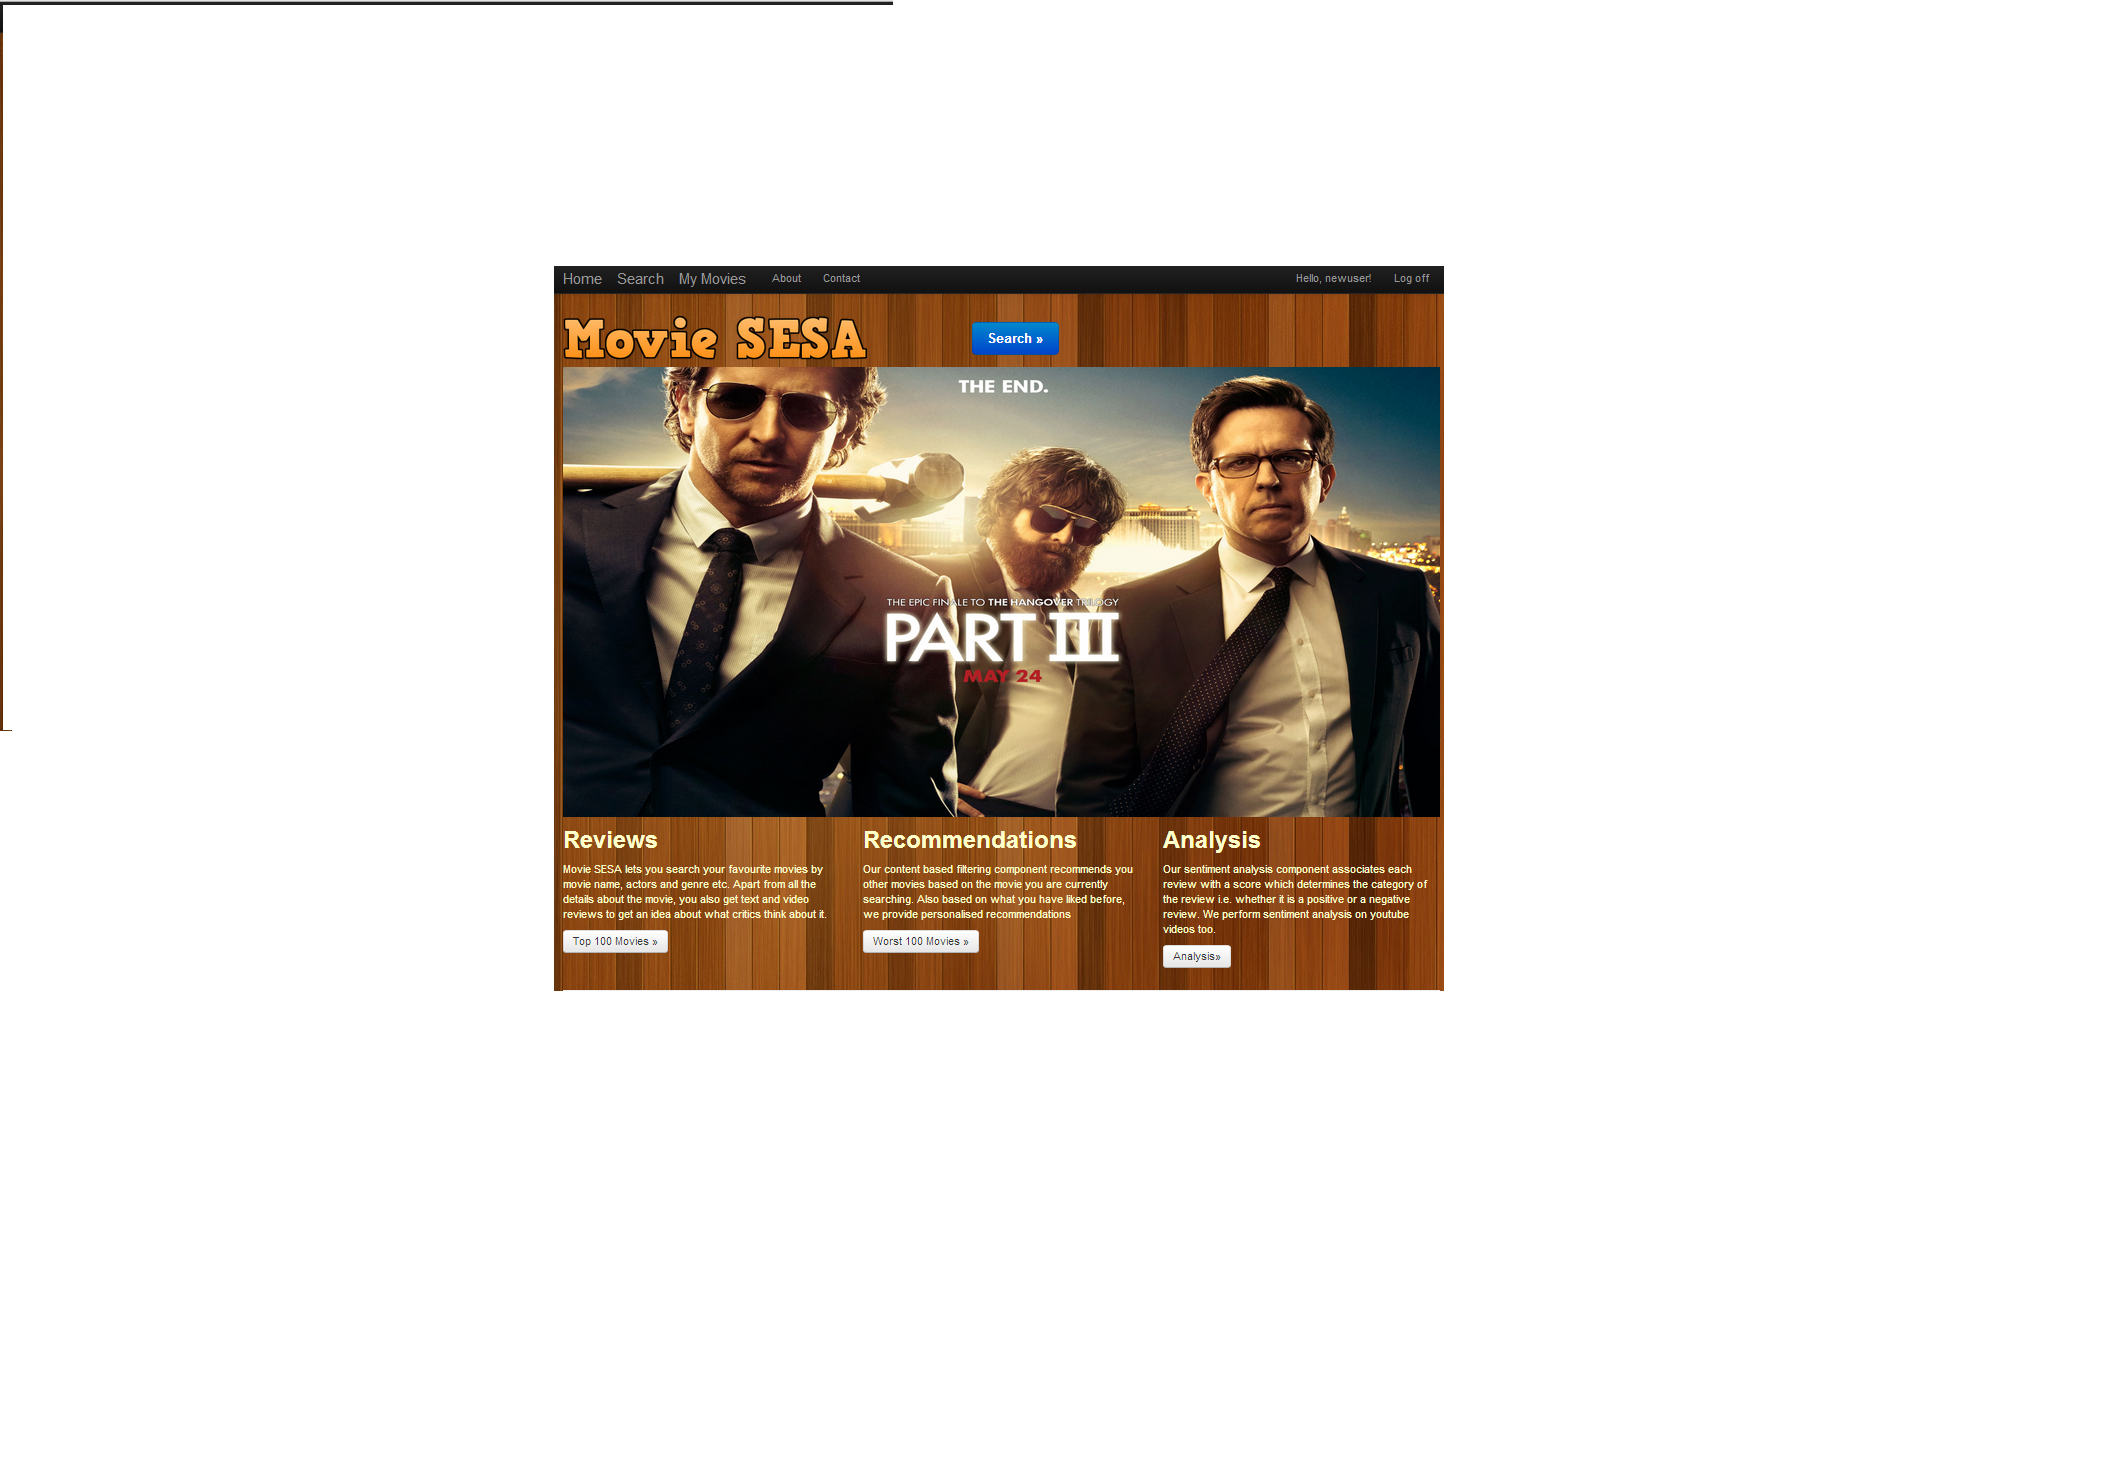
\includegraphics[width=5.0in]{home.png}
    \caption{Different pages in our application}
    \label{fig:home}
\end{figure}

We use 3 tables in our database. Fig\ref{fig:database} shows an intuitive representation of how the databases are used. We put the data from \textit{Movies.xml} to our database table \textit{Movies} and all the movie web pages display their content based on data from this table. We use the clustering data for our content based recommendations. This clustering data are taken from \textit{Clusters.xml} and are put in the database table \textit{clusters}. For user modeling we use the table \textit{UserLikeMovies}. Whenever a user likes a movie, the data is inserted in this table and the user category is evaluated dynamically.
 
\begin{figure}[H]
    \centering
    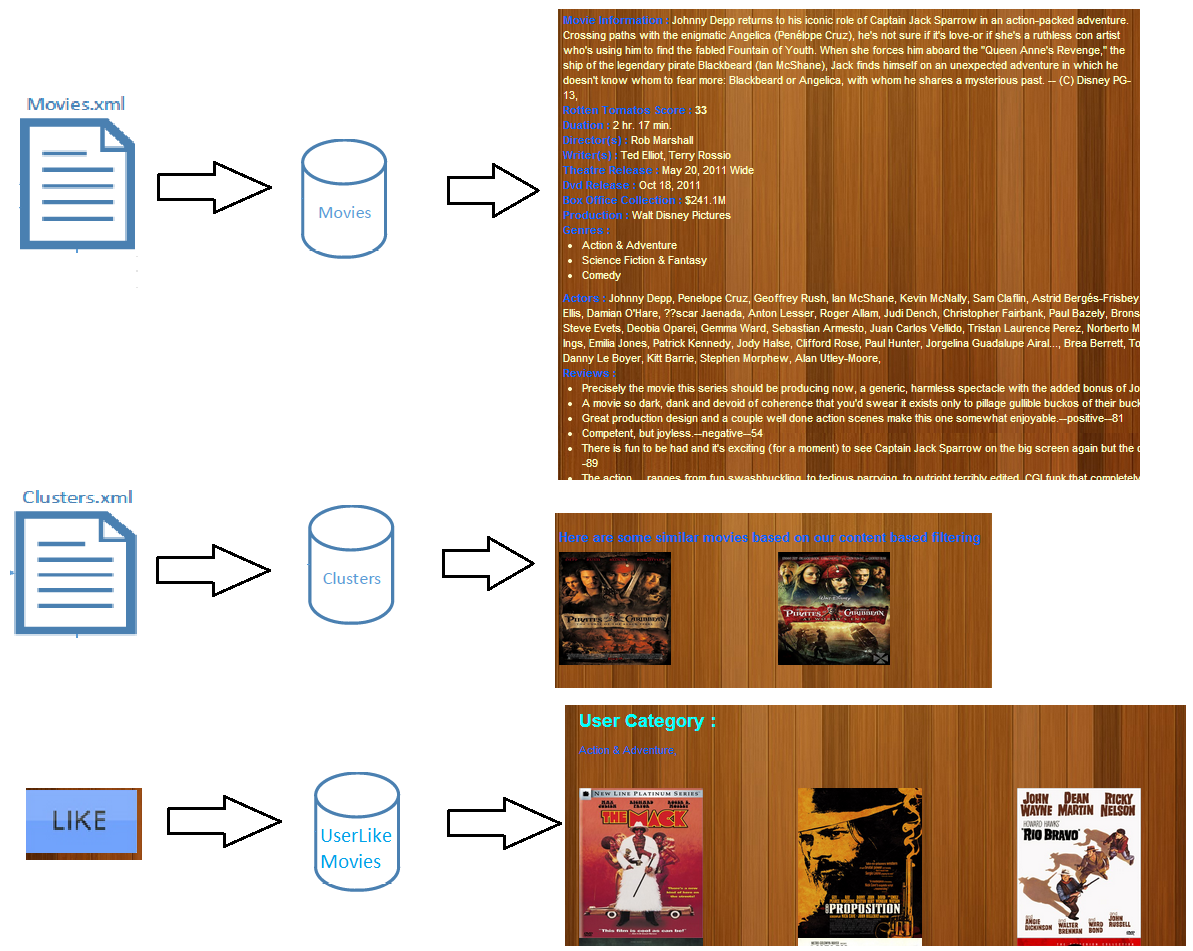
\includegraphics[width=4.0in]{database.png}
    \caption{Databae tables in our application}
    \label{fig:database}
\end{figure}
